\documentclass[../main.tex]{subfiles}
\begin{document}

\begin{definition}\label{def:2.5.1}
    称一个连续型随机变量 $X$ 服从\emph{均匀分布},若其 PDF 为 $f(x)=\frac{1}{b-a}(x\in(a,b))$,$f$ 在其余各处取 $0$。记作 $X\sim U(a,b)$。
\end{definition}

我们常将 $X\sim U(0,1)$ 称为随机数。

计算可得,若 $X\sim U(a,b)$,则 $\mathrm{E}(X)=\frac{a+b}{2},\mathrm{Var}(X)=\frac{(b-a)^2}{12}$。

\begin{definition}\label{def:2.5.2}
    称一个连续型随机变量 $X$ 服从\emph{正态分布},若其 PDF 为 $f(x)=\frac{1}{\sqrt{2\pi}\sigma}e^{-\frac{(x-\mu)^2}{2\sigma^2}}(\sigma>0)$。记作 $X\sim N(\mu,\sigma^2)$。
\end{definition}

计算可得,若 $X\sim N(\mu,\sigma^2)$,则 $\mathrm{E}(X)=\mu,\mathrm{Var}(X)=\sigma^2$。

著名的“经验法则”见图~\ref{fig:2.5.1}。

\begin{figure}[!h]
    \centering
    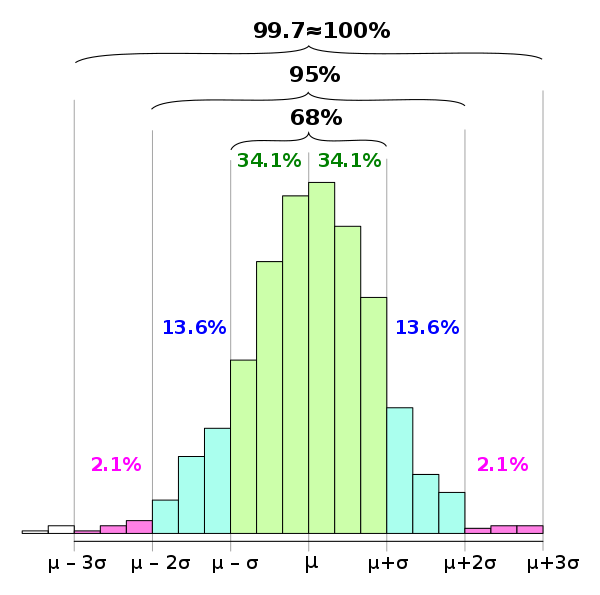
\includegraphics[scale=0.5]{figures/empirical_rule.png}
    \caption{经验法则}
    \label{fig:2.5.1}
\end{figure}

$X\sim N(\mu,\sigma^2)$ 的充要条件是 $Y=\frac{X-\mu}{\sigma}\sim N(0,1)$。我们将 $N(0,1)$ 称为\emph{标准正态分布}。

\begin{definition}\label{def:2.5.3}
    称一个连续型随机变量 $X$ 服从\emph{指数分布},若其 PDF 为 $f(x)=\lambda e^{-\lambda x}(\lambda>0,x>0)$,$f$ 在其余各处取 $0$。记作 $X\sim Exp(\lambda)$。
\end{definition}

指数分布常用于刻画等待时间、寿命等。

计算可得,若 $X\sim Exp(\lambda)$,则 $\mathrm{E}(X)=1/\lambda,\mathrm{Var}(X)=1/\lambda^2$。

指数分布有另一种符号约定,以 $\beta=1/\lambda$ 为参数,一些数学软件可能采用此种约定。

指数分布的 CDF 为 $F(x)=1-e^{-\lambda x}(x>0)$,所谓的“尾概率”为 $P(X>x)=1-F(x)=e^{-\lambda x}(x>0)$。

\begin{example}
    设某医院平均每天出生婴儿数为 $\lambda$,现在观察到一名婴儿出生,则接下来 $t$ 天内有婴儿出生的概率为 $P(X\leq t)$,其中 $X$ 表示到下一个婴儿出生所需等待的时间。\\
    记 $N(t)$ 为 $t$ 天内出生婴儿数,我们已经知道 $N(t)\sim P(t\lambda)$,则 $P(X>t)=P(N(t)=0)=e^{-\lambda t}$,故 $P(X\leq t)=1-e^{-\lambda t}$。我们发现 $X$ 服从参数为 $\lambda$ 的指数分布。
\end{example}

我们从另一个角度理解指数分布。

首先引入\emph{失效率}或\emph{危险率}的概念。设 $X$ 为连续型随机变量(表示某种零件的寿命),其 CDF 为 $F(x)$,且 $F(0)=0$。考虑条件概率 $P(x<X<x+\mathrm{d}x|X>x)=\frac{P(x<X<x+\mathrm{d}x)}{P(X>x)}=\frac{F(x+\mathrm{d}x)-F(x)}{1-F(x)}\approx\frac{F^\prime(x)}{1-F(x)}\mathrm{d}x$,即“年龄”为 $x$ 的零件不能继续工作的条件概率密度为 $\frac{F^\prime(x)}{1-F(x)}$,我们称其为瞬时失效率 $\lambda(x)$,则 $F(x)=1-e^{-\int_0^x\lambda(t)\mathrm{d}t}$。

在“无老化”假设下,即 $\lambda(t)\equiv \lambda$ 不随时间变化,则 $F(x)=1-e^{-\lambda t}(x>0)$,$X$ 服从指数分布。

指数分布有所谓“无记忆性”:$P(X>t+s|X>s)=\frac{P(X>t+s)}{P(X>s)}=e^{-\lambda t}=P(X>t)(t,s>0)$。

“无老化”假设并不总是成立。为此,我们可以进行一定程度的改进,例如令 $\lambda(x)=\alpha\frac{x^{\alpha-1}}{\beta^\alpha}(x>0,\alpha,\beta>0\text{ 为常数})$,则 $F(x)=1-e^{-(\frac{x}{\beta})^\alpha}(x>0)$,称之为 \emph{Weibull 分布}。当 $\alpha=1$ 时,Weibull 分布退化为参数为 $1/\beta$ 的指数分布。

总览至此我们介绍过的各个分布的参数,可以将其大致分为以下几类:
\begin{enumerate}
    \item 位置参数:决定了分布平移到的位置,通常在 PMF/PDF 中体现为 $f(x)=g(x-\cdot)$ 的形式,如正态分布的参数 $\mu$
    \item 尺度参数:决定了分布伸缩的程度,通常在 PMF/PDF 中体现为 $f(x)=g(\frac x\cdot)$ 的形式,如正态分布的参数 $\sigma$、Weibull 分布的参数 $\beta$
    \item 形状参数:决定了分布的形状,如 Weibull 分布的参数 $\alpha$
\end{enumerate}

\end{document}
